%% Copyright 2005 G. W. Knor
%%This work may be distributed and/or modified under the
% conditions of the LaTeX Project Public License, either version 1.3
% of this license or (at your option) any later version.
% The latest version of this license is in
% http://www.latex-project.org/lppl.txt
% and version 1.3 or later is part of all distributions of LaTeX
% version 2005/12/01 or later.
%%This work has the LPPL maintenance status "maintained".
%%The Current Maintainer of this work is G. W. Knor.
 
\documentclass{beamer}
\usepackage{graphicx}
\usepackage{amsmath} % provides \text{<stuff>} which prints <stuff> in text mode
\usepackage{sidecap}
\usepackage{courier}
\usepackage{listings}
\usepackage{hyperref}
\usepackage[utf8]
{inputenc}
\lstset{
    breaklines=true,
    breakatwhitespace=true,
    postbreak=\raisebox{0ex}[0ex][0ex]{\ensuremath{\color{red}\hookrightarrow\space}}
}
\setcounter{tocdepth}{1}

\definecolor{keywords}{RGB}{255,0,90}
\definecolor{comments}{RGB}{0,0,113}
\definecolor{red}{RGB}{160,0,0}
\definecolor{green}{RGB}{0,150,0}
 
\lstset{language=Python, 
        basicstyle=\ttfamily\small, 
        keywordstyle=\color{keywords},
        commentstyle=\color{comments},
        stringstyle=\color{red},
        showstringspaces=false,
        identifierstyle=\color{green},
        procnamekeys={def,class}}


\title{HowTo re}
\author{Dariusz Śmigiel}
\date{PyCon PL 2015}
\usetheme{Warsaw}
\usecolortheme{beaver}

\begin{document}

\begin{frame}
\titlepage
\end{frame}

\section{History}
\subsection{Origins}
\begin{frame}
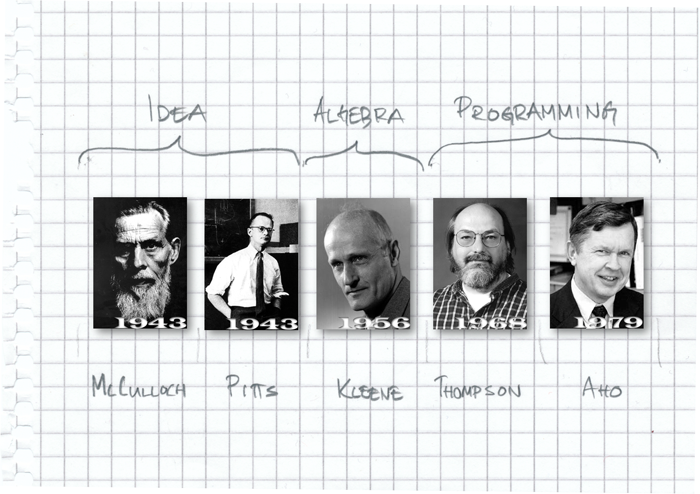
\includegraphics[width=1\textwidth]{images/history.png}
\end{frame}

\subsection{re module}
\begin{frame}
Delivering Quality since December 31, 1997 \\
\pause
Release of Python 1.5
\pause

\begin{itemize}
 \item Deprecated old module `regex`, based on Perl-style patterns.
\pause
 \item `regex` finally removed in Python 2.5.
\end{itemize}
\end{frame}

\section{Do I need it?}
\subsection{Matching}
\begin{frame}
Answer for questions:
 \begin{itemize}
  \item "Does this string match the pattern?"
  \item "Is there a match for the pattern anywhere in this string?"
 \end{itemize}
\end{frame}

\subsection{Modifying}
\begin{frame}
\begin{itemize}
\item Replace part of it
\item Split into pieces
\end{itemize}
\end{frame}

\section{Under the hood}
\subsection{Implementation}
\begin{frame}
 \structure{\insertsubsection}
re patterns are compiled into bytecode \\
\pause
executed by engine written in C

\subsection{Features}
 \structure{\insertsubsection}
re language is relatively small and restricted
\pause
 \begin{itemize}
  \item not all possible string processing tasks can be done
  \item some of them can be done, but expression would be very complicated
 \end{itemize}
\end{frame}

\begin{frame}[fragile]
\begingroup
 \fontsize{6pt}{8pt}\selectfont
\begin{verbatim}
(?:(?:\r\n)?[ \t])*(?:(?:(?:[^()<>@,;:\\".\[\] \000-\031]+(?:(?:(?:\r\n)?[ \t]
)+|\Z|(?=[\["()<>@,;:\\".\[\]]))|"(?:[^\"\r\\]|\\.|(?:(?:\r\n)?[ \t]))*"(?:(?:
\r\n)?[ \t])*)(?:\.(?:(?:\r\n)?[ \t])*(?:[^()<>@,;:\\".\[\] \000-\031]+(?:(?:(
?:\r\n)?[ \t])+|\Z|(?=[\["()<>@,;:\\".\[\]]))|"(?:[^\"\r\\]|\\.|(?:(?:\r\n)?[ 
\t]))*"(?:(?:\r\n)?[ \t])*))*@(?:(?:\r\n)?[ \t])*(?:[^()<>@,;:\\".\[\] \000-\0
31]+(?:(?:(?:\r\n)?[ \t])+|\Z|(?=[\["()<>@,;:\\".\[\]]))|\[([^\[\]\r\\]|\\.)*\
](?:(?:\r\n)?[ \t])*)(?:\.(?:(?:\r\n)?[ \t])*(?:[^()<>@,;:\\".\[\] \000-\031]+
(?:(?:(?:\r\n)?[ \t])+|\Z|(?=[\["()<>@,;:\\".\[\]]))|\[([^\[\]\r\\]|\\.)*\](?:
(?:\r\n)?[ \t])*))*|(?:[^()<>@,;:\\".\[\] \000-\031]+(?:(?:(?:\r\n)?[ \t])+|\Z
|(?=[\["()<>@,;:\\".\[\]]))|"(?:[^\"\r\\]|\\.|(?:(?:\r\n)?[ \t]))*"(?:(?:\r\n)
?[ \t])*)*\<(?:(?:\r\n)?[ \t])*(?:@(?:[^()<>@,;:\\".\[\] \000-\031]+(?:(?:(?:\
r\n)?[ \t])+|\Z|(?=[\["()<>@,;:\\".\[\]]))|\[([^\[\]\r\\]|\\.)*\](?:(?:\r\n)?[
 \t])*)(?:\.(?:(?:\r\n)?[ \t])*(?:[^()<>@,;:\\".\[\] \000-\031]+(?:(?:(?:\r\n)
?[ \t])+|\Z|(?=[\["()<>@,;:\\".\[\]]))|\[([^\[\]\r\\]|\\.)*\](?:(?:\r\n)?[ \t]
)*))*(?:,@(?:(?:\r\n)?[ \t])*(?:[^()<>@,;:\\".\[\] \000-\031]+(?:(?:(?:\r\n)?[
 \t])+|\Z|(?=[\["()<>@,;:\\".\[\]]))|\[([^\[\]\r\\]|\\.)*\](?:(?:\r\n)?[ \t])*
)(?:\.(?:(?:\r\n)?[ \t])*(?:[^()<>@,;:\\".\[\] \000-\031]+(?:(?:(?:\r\n)?[ \t]
)+|\Z|(?=[\["()<>@,;:\\".\[\]]))|\[([^\[\]\r\\]|\\.)*\](?:(?:\r\n)?[ \t])*))*)
*:(?:(?:\r\n)?[ \t])*)?(?:[^()<>@,;:\\".\[\] \000-\031]+(?:(?:(?:\r\n)?[ \t])+
|\Z|(?=[\["()<>@,;:\\".\[\]]))|"(?:[^\"\r\\]|\\.|(?:(?:\r\n)?[ \t]))*"(?:(?:\r
\n)?[ \t])*)(?:\.(?:(?:\r\n)?[ \t])*(?:[^()<>@,;:\\".\[\] \000-\031]+(?:(?:(?:
\end{verbatim}
 \endgroup
\end{frame}

\begin{frame}[fragile]
\begingroup
 \fontsize{6pt}{8pt}\selectfont
\begin{verbatim}
\r\n)?[ \t])+|\Z|(?=[\["()<>@,;:\\".\[\]]))|"(?:[^\"\r\\]|\\.|(?:(?:\r\n)?[ \t
]))*"(?:(?:\r\n)?[ \t])*))*@(?:(?:\r\n)?[ \t])*(?:[^()<>@,;:\\".\[\] \000-\031
]+(?:(?:(?:\r\n)?[ \t])+|\Z|(?=[\["()<>@,;:\\".\[\]]))|\[([^\[\]\r\\]|\\.)*\](
?:(?:\r\n)?[ \t])*)(?:\.(?:(?:\r\n)?[ \t])*(?:[^()<>@,;:\\".\[\] \000-\031]+(?
:(?:(?:\r\n)?[ \t])+|\Z|(?=[\["()<>@,;:\\".\[\]]))|\[([^\[\]\r\\]|\\.)*\](?:(?
:\r\n)?[ \t])*))*\>(?:(?:\r\n)?[ \t])*)|(?:[^()<>@,;:\\".\[\] \000-\031]+(?:(?
:(?:\r\n)?[ \t])+|\Z|(?=[\["()<>@,;:\\".\[\]]))|"(?:[^\"\r\\]|\\.|(?:(?:\r\n)?
[ \t]))*"(?:(?:\r\n)?[ \t])*)*:(?:(?:\r\n)?[ \t])*(?:(?:(?:[^()<>@,;:\\".\[\] 
\000-\031]+(?:(?:(?:\r\n)?[ \t])+|\Z|(?=[\["()<>@,;:\\".\[\]]))|"(?:[^\"\r\\]|
\\.|(?:(?:\r\n)?[ \t]))*"(?:(?:\r\n)?[ \t])*)(?:\.(?:(?:\r\n)?[ \t])*(?:[^()<>
@,;:\\".\[\] \000-\031]+(?:(?:(?:\r\n)?[ \t])+|\Z|(?=[\["()<>@,;:\\".\[\]]))|"
(?:[^\"\r\\]|\\.|(?:(?:\r\n)?[ \t]))*"(?:(?:\r\n)?[ \t])*))*@(?:(?:\r\n)?[ \t]
)*(?:[^()<>@,;:\\".\[\] \000-\031]+(?:(?:(?:\r\n)?[ \t])+|\Z|(?=[\["()<>@,;:\\
".\[\]]))|\[([^\[\]\r\\]|\\.)*\](?:(?:\r\n)?[ \t])*)(?:\.(?:(?:\r\n)?[ \t])*(?
:[^()<>@,;:\\".\[\] \000-\031]+(?:(?:(?:\r\n)?[ \t])+|\Z|(?=[\["()<>@,;:\\".\[
\]]))|\[([^\[\]\r\\]|\\.)*\](?:(?:\r\n)?[ \t])*))*|(?:[^()<>@,;:\\".\[\] \000-
\031]+(?:(?:(?:\r\n)?[ \t])+|\Z|(?=[\["()<>@,;:\\".\[\]]))|"(?:[^\"\r\\]|\\.|(
?:(?:\r\n)?[ \t]))*"(?:(?:\r\n)?[ \t])*)*\<(?:(?:\r\n)?[ \t])*(?:@(?:[^()<>@,;
:\\".\[\] \000-\031]+(?:(?:(?:\r\n)?[ \t])+|\Z|(?=[\["()<>@,;:\\".\[\]]))|\[([
^\[\]\r\\]|\\.)*\](?:(?:\r\n)?[ \t])*)(?:\.(?:(?:\r\n)?[ \t])*(?:[^()<>@,;:\\"
.\[\] \000-\031]+(?:(?:(?:\r\n)?[ \t])+|\Z|(?=[\["()<>@,;:\\".\[\]]))|\[([^\[\
\end{verbatim}
 \endgroup
\end{frame}

\begin{frame}[fragile]
\begingroup
 \fontsize{6pt}{8pt}\selectfont
\begin{verbatim}
]\r\\]|\\.)*\](?:(?:\r\n)?[ \t])*))*(?:,@(?:(?:\r\n)?[ \t])*(?:[^()<>@,;:\\".\
[\] \000-\031]+(?:(?:(?:\r\n)?[ \t])+|\Z|(?=[\["()<>@,;:\\".\[\]]))|\[([^\[\]\
r\\]|\\.)*\](?:(?:\r\n)?[ \t])*)(?:\.(?:(?:\r\n)?[ \t])*(?:[^()<>@,;:\\".\[\] 
\000-\031]+(?:(?:(?:\r\n)?[ \t])+|\Z|(?=[\["()<>@,;:\\".\[\]]))|\[([^\[\]\r\\]
|\\.)*\](?:(?:\r\n)?[ \t])*))*)*:(?:(?:\r\n)?[ \t])*)?(?:[^()<>@,;:\\".\[\] \0
00-\031]+(?:(?:(?:\r\n)?[ \t])+|\Z|(?=[\["()<>@,;:\\".\[\]]))|"(?:[^\"\r\\]|\\
.|(?:(?:\r\n)?[ \t]))*"(?:(?:\r\n)?[ \t])*)(?:\.(?:(?:\r\n)?[ \t])*(?:[^()<>@,
;:\\".\[\] \000-\031]+(?:(?:(?:\r\n)?[ \t])+|\Z|(?=[\["()<>@,;:\\".\[\]]))|"(?
:[^\"\r\\]|\\.|(?:(?:\r\n)?[ \t]))*"(?:(?:\r\n)?[ \t])*))*@(?:(?:\r\n)?[ \t])*
(?:[^()<>@,;:\\".\[\] \000-\031]+(?:(?:(?:\r\n)?[ \t])+|\Z|(?=[\["()<>@,;:\\".
\[\]]))|\[([^\[\]\r\\]|\\.)*\](?:(?:\r\n)?[ \t])*)(?:\.(?:(?:\r\n)?[ \t])*(?:[
^()<>@,;:\\".\[\] \000-\031]+(?:(?:(?:\r\n)?[ \t])+|\Z|(?=[\["()<>@,;:\\".\[\]
]))|\[([^\[\]\r\\]|\\.)*\](?:(?:\r\n)?[ \t])*))*\>(?:(?:\r\n)?[ \t])*)(?:,\s*(
?:(?:[^()<>@,;:\\".\[\] \000-\031]+(?:(?:(?:\r\n)?[ \t])+|\Z|(?=[\["()<>@,;:\\
".\[\]]))|"(?:[^\"\r\\]|\\.|(?:(?:\r\n)?[ \t]))*"(?:(?:\r\n)?[ \t])*)(?:\.(?:(
?:\r\n)?[ \t])*(?:[^()<>@,;:\\".\[\] \000-\031]+(?:(?:(?:\r\n)?[ \t])+|\Z|(?=[
\["()<>@,;:\\".\[\]]))|"(?:[^\"\r\\]|\\.|(?:(?:\r\n)?[ \t]))*"(?:(?:\r\n)?[ \t
])*))*@(?:(?:\r\n)?[ \t])*(?:[^()<>@,;:\\".\[\] \000-\031]+(?:(?:(?:\r\n)?[ \t
])+|\Z|(?=[\["()<>@,;:\\".\[\]]))|\[([^\[\]\r\\]|\\.)*\](?:(?:\r\n)?[ \t])*)(?
:\.(?:(?:\r\n)?[ \t])*(?:[^()<>@,;:\\".\[\] \000-\031]+(?:(?:(?:\r\n)?[ \t])+|
\Z|(?=[\["()<>@,;:\\".\[\]]))|\[([^\[\]\r\\]|\\.)*\](?:(?:\r\n)?[ \t])*))*|(?:
\end{verbatim}
 \endgroup
\end{frame}

\begin{frame}[fragile]
\begingroup
 \fontsize{6pt}{8pt}\selectfont
\begin{verbatim}
[^()<>@,;:\\".\[\] \000-\031]+(?:(?:(?:\r\n)?[ \t])+|\Z|(?=[\["()<>@,;:\\".\[\
]]))|"(?:[^\"\r\\]|\\.|(?:(?:\r\n)?[ \t]))*"(?:(?:\r\n)?[ \t])*)*\<(?:(?:\r\n)
?[ \t])*(?:@(?:[^()<>@,;:\\".\[\] \000-\031]+(?:(?:(?:\r\n)?[ \t])+|\Z|(?=[\["
()<>@,;:\\".\[\]]))|\[([^\[\]\r\\]|\\.)*\](?:(?:\r\n)?[ \t])*)(?:\.(?:(?:\r\n)
?[ \t])*(?:[^()<>@,;:\\".\[\] \000-\031]+(?:(?:(?:\r\n)?[ \t])+|\Z|(?=[\["()<>
@,;:\\".\[\]]))|\[([^\[\]\r\\]|\\.)*\](?:(?:\r\n)?[ \t])*))*(?:,@(?:(?:\r\n)?[
 \t])*(?:[^()<>@,;:\\".\[\] \000-\031]+(?:(?:(?:\r\n)?[ \t])+|\Z|(?=[\["()<>@,
;:\\".\[\]]))|\[([^\[\]\r\\]|\\.)*\](?:(?:\r\n)?[ \t])*)(?:\.(?:(?:\r\n)?[ \t]
)*(?:[^()<>@,;:\\".\[\] \000-\031]+(?:(?:(?:\r\n)?[ \t])+|\Z|(?=[\["()<>@,;:\\
".\[\]]))|\[([^\[\]\r\\]|\\.)*\](?:(?:\r\n)?[ \t])*))*)*:(?:(?:\r\n)?[ \t])*)?
(?:[^()<>@,;:\\".\[\] \000-\031]+(?:(?:(?:\r\n)?[ \t])+|\Z|(?=[\["()<>@,;:\\".
\[\]]))|"(?:[^\"\r\\]|\\.|(?:(?:\r\n)?[ \t]))*"(?:(?:\r\n)?[ \t])*)(?:\.(?:(?:
\r\n)?[ \t])*(?:[^()<>@,;:\\".\[\] \000-\031]+(?:(?:(?:\r\n)?[ \t])+|\Z|(?=[\[
"()<>@,;:\\".\[\]]))|"(?:[^\"\r\\]|\\.|(?:(?:\r\n)?[ \t]))*"(?:(?:\r\n)?[ \t])
*))*@(?:(?:\r\n)?[ \t])*(?:[^()<>@,;:\\".\[\] \000-\031]+(?:(?:(?:\r\n)?[ \t])
+|\Z|(?=[\["()<>@,;:\\".\[\]]))|\[([^\[\]\r\\]|\\.)*\](?:(?:\r\n)?[ \t])*)(?:\
.(?:(?:\r\n)?[ \t])*(?:[^()<>@,;:\\".\[\] \000-\031]+(?:(?:(?:\r\n)?[ \t])+|\Z
|(?=[\["()<>@,;:\\".\[\]]))|\[([^\[\]\r\\]|\\.)*\](?:(?:\r\n)?[ \t])*))*\>(?:(
?:\r\n)?[ \t])*))*)?;\s*)
\end{verbatim}
 \endgroup
Perl regex to validate email addresses according to the RFC 822
\url{http://ex-parrot.com/~pdw/Mail-RFC822-Address}
\end{frame}

\section{Simple patterns}
\subsection{Metacharacters}
\begin{frame}[fragile]
\begin{verbatim}
. ^ $ * + ? { } [ ] \ | ( )
\end{verbatim}
\end{frame}

\subsubsection{Class}
\begin{frame}[fragile]
\begin{verbatim}
[ ]
\end{verbatim}
Specifying a character class, which is set of characters that you wish to match
 \begin{itemize}
  \item can be listed individually \verb/[abc]/
  \item can be given as range of characters, separated by '-' \verb/[a-c]/
 \end{itemize}
\pause
Metacharacters are not active inside class \\
\verb/[akm$]/ will match any of: "a", "k", "m", "\$"
\end{frame}

\subsubsection{Complementing set}
\begin{frame}[fragile]
\begin{verbatim}
^
\end{verbatim}
Including \verb/^/ as first character of the class \verb/[^5]/ will match any except '5'
\end{frame}

\subsubsection{Backslash - escape metacharacters}
\begin{frame}[fragile]
\begin{verbatim}
\
\end{verbatim}
For matching \verb/[/ or \verb/\/ you can use \verb/\[/ or \verb/\\/
\pause
Some of special sequences beginning with \verb/\/ express predefined sets of characters: set of digits, letters, everything but whitespace
\end{frame}

\begin{frame}[fragile]
\begin{itemize}
\item \verb/\d/ - any decimal digit, equivalent of \verb/[0-9]/
\item \verb/\D/ - everything but decimal digit, equivalent of \verb/[^0-9]/
\pause
\item \verb/\w/ - any alphanumeric: \verb/[a-zA-Z0-9_]/
\item \verb/\W/ - any non-alpahnumeric: \verb/[^a-zA-Z0-9_]/
\pause
\item \verb/\s/ - any whitespace character: \verb/[ \t\n\r\f\v]/ \\ (space, tab (ASCII 0x09), newline (0x0A), return (0x0D), form feed - page break(0x0C), vertical tab (0x0B))
\item \verb/\S/ - any non-whitespace character: \verb/[^ \t\n\r\f\v]/
\\
NOTE! Remember that Windows text files use \verb/\r\n/ to terminate lines, while UNIX text files use \verb/\n/.
\end{itemize}
\end{frame}

\subsubsection{Dot - '.'}
\begin{frame}[fragile]
\begin{verbatim}
.
\end{verbatim}
By default, matches anything except newline character.
\pause
There is alternate mode (re.DOTALL) where it matches everything. Used when it's needed to match "any character"
\end{frame}

\subsection{Repeating Things}
\subsubsection{Star - "*"}
\begin{frame}[fragile]
\begin{verbatim}
*
\end{verbatim}
Doesn't match a character. Specifies that previous character can be matched zero or more times.
\begin{verbatim}
(ca*t) --> "ct", "cat", "caaat"
\end{verbatim}
NOTE! RE engine has limitations stemming from the size of C's \verb/int/ type that will prevent it from matching over 2 billion \verb/a/ characters (2GB).
\end{frame}

\begin{frame}[fragile]
\verb/*/ is greedy -- will try to repeat it as many times as possible \\
\verb/a[bcd]*b/ - matches \verb/a/, zero or more letters from \verb/bcd/, and ends with \verb/b/ \\
\verb/abcbd/
\begin{itemize}
\item matches \verb/a/
\item matches \verb/abcbd/ to the end of the string
\item fails, because current position is the end of the string, so cannot match \verb/b/
\item matches \verb/abcb/ - one less character
\item fails, because current position is \verb/d/, so cannot match \verb/b/
\item matches \verb/abc/, so \verb/[bcd]*/ matches only \verb/bc/
\item \verb/abcb/, tries last character \verb/b/, and it's on current position
\item success
\end{itemize}
\end{frame}

\subsubsection{Plus -- "+"}
\begin{verbatim}
+
\end{verbatim}
\begin{frame}[fragile]
Similar to "*", but requires at least one occurence of character
\begin{verbatim}
(ca+t) --> "cat", "caaat" but not "ct"
\end{verbatim}
\end{frame}

\subsubsection{Quotation mark -- "?"}
\begin{frame}[fragile]
\begin{verbatim}
?
\end{verbatim}
Matches either once or zero times
\begin{verbatim}
(home-?brew) --> "homebrew", "home-brew"
\end{verbatim}
\end{frame}

\subsubsection{"{m,n}"}
\begin{frame}[fragile]
"m" and "n" are decimal numbers. There must be at least m repetitions, and at most n.
\begin{verbatim}
a/{1,3}b --> a/b, a//b, a///b
\end{verbatim}
\pause
m and n can be ommited. When m ommited, there is zero, when n ommited, upper bound infinity (more precisely, 2 billions)
\end{frame}

\subsubsection{Equivalents}
\begin{frame}[fragile]
\begin{verbatim}
{0,} == "*"
{1,} == "+"
{,1} == {0,1} == "?"
\end{verbatim}
\end{frame}

\section{Regular Expressions}
\begin{frame}
REs are handled as strings because regular expressions aren’t part of the core Python language, and no special syntax was created for expressing them. \\
(There are applications that don’t need REs at all, so there’s no need to bloat the language specification by including them.) \\ 
Instead, the re module is simply a C extension module included with Python, just like the socket or zlib modules. \\
\end{frame}

\begin{frame}[fragile]
\begin{verbatim}
Backslash Plague

Characters	Stage
\section	Text string to be matched
\\section	Escaped backslash for re.compile()
"\\\\section"	Escaped backslashes for a string literal

to match a literal backslash, one has to write '\\\\' as the RE string, because the regular expression must be \\, and each backslash must be expressed as \\ inside a regular Python string literal.

Solution
Regular String	Raw string
"ab*"	r"ab*"
"\\\\section"	r"\\section"
"\\w+\\s+\\1"	r"\w+\s+\1"
\end{verbatim}
\end{frame}


\section{Bibliography}
\begin{frame}
Regular Expression HOWTO: \url{https://docs.python.org/2/howto/regex.html}
Python Docs: Library re: \url{https://docs.python.org/2/library/re.html}
Google for Education. Python Regular Expressions: \url{https://developers.google.com/edu/python/regular-expressions?hl=en}
Non-printable Characters: \url{http://www.regular-expressions.info/nonprint.html}
Core Python Applications programming: Regular expressions: \url{http://www.informit.com/articles/article.aspx?p=1707750&seqNum=2}
Brief history by Staffan Noteberg: \url{http://blog.staffannoteberg.com/}
\end{frame}
\end{document}
